% Autor: Matheus Sousa, Labotatório de Comunicação e Segurança da Informação, DES-CTG, UFPE.
\documentclass{article}
\usepackage[a4paper, landscape, margin=1.2cm]{geometry}
\usepackage{tikz}
\usepackage{caption}
\usepackage{subcaption}
\usepackage{amsmath,amssymb}
\usetikzlibrary{shapes.symbols, arrows.meta, calc}
% Autor: Matheus Sousa, Labotatório de Comunicação e Segurança da Informação, DES-CTG, UFPE.
\tikzset{
  rtl/.style    = {font=\footnotesize, line width=0.5pt, >={Stealth[length=1.6mm]}},
  bloco/.style  = {draw, minimum width=11mm, minimum height=8mm, inner sep=1pt, align=center},
  porta/.style  = {draw, signal, signal to=east, minimum height=4.5mm,
                   minimum width=9mm, inner sep=1pt, font=\scriptsize},
  nivel/.style  = {draw, circle, minimum size=5mm, inner sep=0pt},
  barra/.style  = {font=\scriptsize, inner sep=1pt},
  no/.style     = {circle, fill, inner sep=0pt, minimum size=1.3mm},
}

\newcommand{\XOR}[2]{%
  \node[draw, circle, minimum size=5mm, inner sep=0pt] (#1) at (#2) {};
  \draw (#1.north) -- (#1.south) (#1.west) -- (#1.east);}

\newcommand{\NOT}[2]{%
  \coordinate (#1) at (#2);
  \draw ($(#1)+(-0.3,0.28)$) -- ($(#1)+(-0.3,-0.28)$) -- ($(#1)+(0.18,0)$) -- cycle;
  \draw ($(#1)+(0.25,0)$) circle (0.07);
  \coordinate (#1-in)  at ($(#1)+(-0.3,0)$);
  \coordinate (#1-out) at ($(#1)+(0.32,0)$);}

\newcommand{\AND}[2]{%
  \coordinate (#1) at (#2);
  \draw ($(#1)+(-0.35,0.35)$) -- ($(#1)+(0,0.35)$) arc (90:-90:0.35)
        -- ($(#1)+(-0.35,-0.35)$) -- cycle;
  \coordinate (#1-in1) at ($(#1)+(-0.35,0.18)$);
  \coordinate (#1-in0) at ($(#1)+(-0.35,-0.18)$);
  \coordinate (#1-out) at ($(#1)+(0.35,0)$);}

\newcommand{\MUX}[2]{%
  \coordinate (#1) at (#2);
  \draw ($(#1)+(-0.35,0.8)$) -- ($(#1)+(0.35,0.45)$) -- ($(#1)+(0.35,-0.45)$)
        -- ($(#1)+(-0.35,-0.8)$) -- cycle;
  \coordinate (#1-in1) at ($(#1)+(-0.35,0.4)$);
  \coordinate (#1-in0) at ($(#1)+(-0.35,-0.4)$);
  \coordinate (#1-sel) at ($(#1)+(0,-0.63)$);
  \coordinate (#1-out) at ($(#1)+(0.35,0)$);
  \node[font=\scriptsize] at ($(#1)+(-0.2,0.4)$) {1};
  \node[font=\scriptsize] at ($(#1)+(-0.2,-0.4)$) {0};}

\newcommand{\FF}[3]{%
  \coordinate (#1) at (#2);
  \draw ($(#1)+(-0.6,-0.9)$) rectangle ($(#1)+(0.6,0.9)$);
  \draw ($(#1)+(-0.6,-0.45)$) -- ($(#1)+(-0.45,-0.55)$) -- ($(#1)+(-0.6,-0.65)$);
  \node[font=\scriptsize] at ($(#1)+(-0.42,0.4)$) {D};
  \node[font=\scriptsize] at ($(#1)+(0.42,0.4)$) {Q};
  \node[font=\scriptsize, anchor=west] at ($(#1)+(-0.42,-0.55)$) {clk};
  \node[barra, anchor=south] at ($(#1)+(0,0.9)$) {#3};
  \coordinate (#1-d)   at ($(#1)+(-0.6,0.4)$);
  \coordinate (#1-q)   at ($(#1)+(0.6,0.4)$);
  \coordinate (#1-clk) at ($(#1)+(-0.6,-0.55)$);}

\newcommand{\Niveis}[3]{%
  \foreach \x in {#1} \draw[dashed, gray] (\x,#2) -- (\x,#3);}
\newcommand{\NumNivel}[3]{\node[nivel] at (#2,#3) {#1};}

\pagestyle{empty}
\renewcommand{\figurename}{Fig.}

\begin{document}

\begin{figure}[p]
  \centering
  \begin{subfigure}{\linewidth}\centering
    \resizebox{0.74\linewidth}{!}{% Autor: Matheus Sousa, Labotatório de Comunicação e Segurança da Informação, DES-CTG, UFPE.
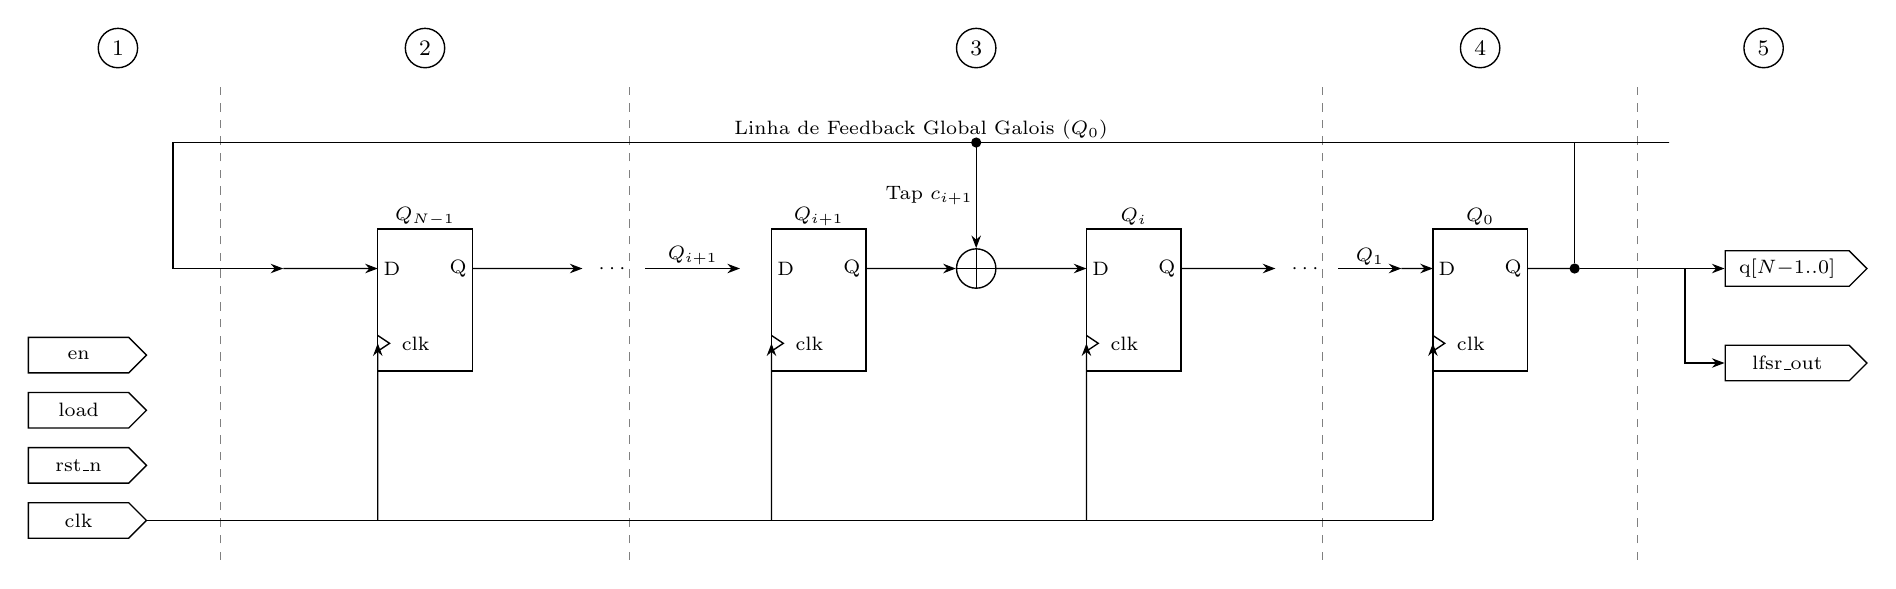
\begin{tikzpicture}[rtl]
  \Niveis{2.6, 7.8, 16.6, 20.6}{-2.5}{3.6}
  \NumNivel{1}{1.3}{4.0}
  \NumNivel{2}{5.2}{4.0}
  \NumNivel{3}{12.2}{4.0}
  \NumNivel{4}{18.6}{4.0}
  \NumNivel{5}{22.2}{4.0}

  \node[porta, minimum width=15mm] (clk)  at (0.8, -2.0) {clk};
  \node[porta, minimum width=15mm] (rst)  at (0.8, -1.3) {rst\_n};
  \node[porta, minimum width=15mm] (load) at (0.8, -0.6) {load};
  \node[porta, minimum width=15mm] (en)   at (0.8,  0.1) {en};

  \FF{ff_msb}{5.2, 0.8}{$Q_{N-1}$}
  \draw[->] (3.4, 1.2) -- (ff_msb-d);

  \draw[->] (ff_msb-q) -- (7.2, 1.2);
  \node[barra] at (7.6, 1.2) {$\cdots$};
  \draw[->] (8.0, 1.2) -- node[barra, above] {$Q_{i+1}$} (9.2, 1.2);

  \FF{ff_ip1}{10.2, 0.8}{$Q_{i+1}$}
  \XOR{xor_i}{12.2, 1.2}
  \draw[->] (ff_ip1-q) -- (xor_i.west);

  \FF{ff_i}{14.2, 0.8}{$Q_i$}
  \draw[->] (xor_i.east) -- (ff_i-d);

  \draw[->] (ff_i-q) -- (16.0, 1.2);
  \node[barra] at (16.4, 1.2) {$\cdots$};
  \draw[->] (16.8, 1.2) -- node[barra, above] {$Q_1$} (17.6, 1.2);

  \FF{ff_0}{18.6, 0.8}{$Q_0$}
  \draw[->] (17.6, 1.2) -- (ff_0-d);

  \draw (ff_0-q) -- (19.8, 1.2) node[no] (node_fb) {};
  \node[porta, minimum width=18mm] (p_q)   at (22.5, 1.2) {q[$N{-}1..0$]};
  \node[porta, minimum width=18mm] (p_out) at (22.5, 0.0) {lfsr\_out};

  \draw[->] (node_fb) -- (p_q.west);
  \draw[->] (node_fb) -| (21.2, 0.0) -- (p_out.west);

  \draw[->] (node_fb) |- (21.0, 2.8) -- (2.0, 2.8) |- (3.4, 1.2);
  \node[barra, above] at (11.5, 2.8) {Linha de Feedback Global Galois ($Q_0$)};

  \draw[->] (12.2, 2.8) node[no] {} -- node[barra, left] {Tap $c_{i+1}$} (xor_i.north);

  \draw (clk.east) -- (18.0, -2.0);
  \draw[->] (4.6, -2.0) -- (ff_msb-clk);
  \draw[->] (9.6, -2.0) -- (ff_ip1-clk);
  \draw[->] (13.6, -2.0) -- (ff_i-clk);
  \draw[->] (18.0, -2.0) -- (ff_0-clk);

\end{tikzpicture}
}
    \caption{Arquitetura RTL geral do LFSR de Galois de $N$ bits com realimentação interna.}
  \end{subfigure}\\[2mm]
  \begin{subfigure}{\linewidth}\centering
    \resizebox{0.68\linewidth}{!}{% Autor: Matheus Sousa, Labotatório de Comunicação e Segurança da Informação, DES-CTG, UFPE.
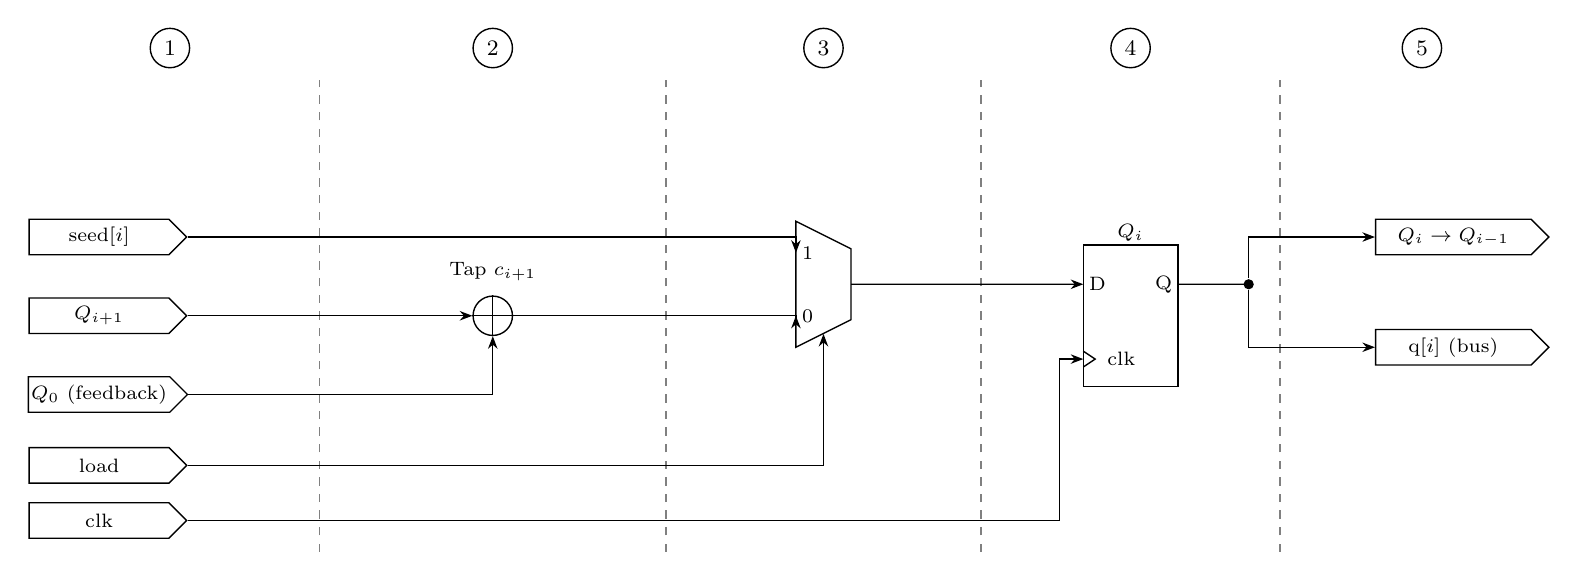
\begin{tikzpicture}[rtl]
  \Niveis{3.8, 8.2, 12.2, 16.0}{-2.6}{3.4}
  \NumNivel{1}{1.9}{3.8}
  \NumNivel{2}{6.0}{3.8}
  \NumNivel{3}{10.2}{3.8}
  \NumNivel{4}{14.1}{3.8}
  \NumNivel{5}{17.8}{3.8}

  \node[porta, minimum width=20mm] (p_seed) at (1.0,  1.4) {seed[$i$]};
  \node[porta, minimum width=20mm] (p_qin)  at (1.0,  0.4) {$Q_{i+1}$};
  \node[porta, minimum width=20mm] (p_fb)   at (1.0, -0.6) {$Q_0$ (feedback)};
  \node[porta, minimum width=20mm] (p_load) at (1.0, -1.5) {load};
  \node[porta, minimum width=20mm] (p_clk)  at (1.0, -2.2) {clk};

  \XOR{xor_tap}{6.0, 0.4}
  \draw[->] (p_qin.east) -- (xor_tap.west);
  \draw[->] (p_fb.east) -| (xor_tap.south);
  \node[barra, above] at (6.0, 0.8) {Tap $c_{i+1}$};

  \MUX{m_load}{10.2, 0.8}
  \draw[->] (p_seed.east) -| (m_load-in1);
  \draw[->] (xor_tap.east) -| (m_load-in0);
  \draw[->] (p_load.east) -| (m_load-sel);

  \FF{ff_cell}{14.1, 0.4}{$Q_i$}
  \draw[->] (m_load-out) -- (ff_cell-d);
  \draw[->] (p_clk.east) -| (13.2, -2.2) |- (ff_cell-clk);

  \draw (ff_cell-q) -- (15.6, 0.8) node[no] (node_cell_out) {};
  \node[porta, minimum width=22mm] (p_qnext) at (18.2,  1.4) {$Q_i \to Q_{i-1}$};
  \node[porta, minimum width=22mm] (p_qbus)  at (18.2,  0.0) {q[$i$] (bus)};

  \draw[->] (node_cell_out) |- (p_qnext.west);
  \draw[->] (node_cell_out) |- (p_qbus.west);

\end{tikzpicture}
}
    \caption{RTL da célula elementar (bit-slice do estágio $i$, repetida para $i = 0, \dots, N-1$).}
  \end{subfigure}
  \caption{Esquemáticos RTL conceituais do LFSR de Galois.
    Em (a), a topologia interna distribui o bit $Q_0$ paralelamente para todos os pontos de tap.
    Nível 1: barramento de controle e realimentação;
    Nível 2: cálculo combinacional do tap com porta XOR ($D_i = Q_{i+1} \oplus Q_0$);
    Nível 3: MUX $2\times1$ para carga síncrona de semente (load);
    Nível 4: registrador de estado Flip-Flop tipo D com clock;
    Nível 5: barramento de saída de estado $q[N{-}1..0]$ e saída serial pseudoaleatória $lfsr\_out = Q_0$.
    Em (b), detalhe de cada estágio individual com seleção condicional do tap $c_{i+1}$.}
  \label{fig:rtl_galois_conceitual}
\end{figure}

\begin{figure}[p]
  \centering
  \begin{subfigure}{\linewidth}\centering
    \resizebox{0.78\linewidth}{!}{% Autor: Matheus Sousa, Labotatório de Comunicação e Segurança da Informação, DES-CTG, UFPE.
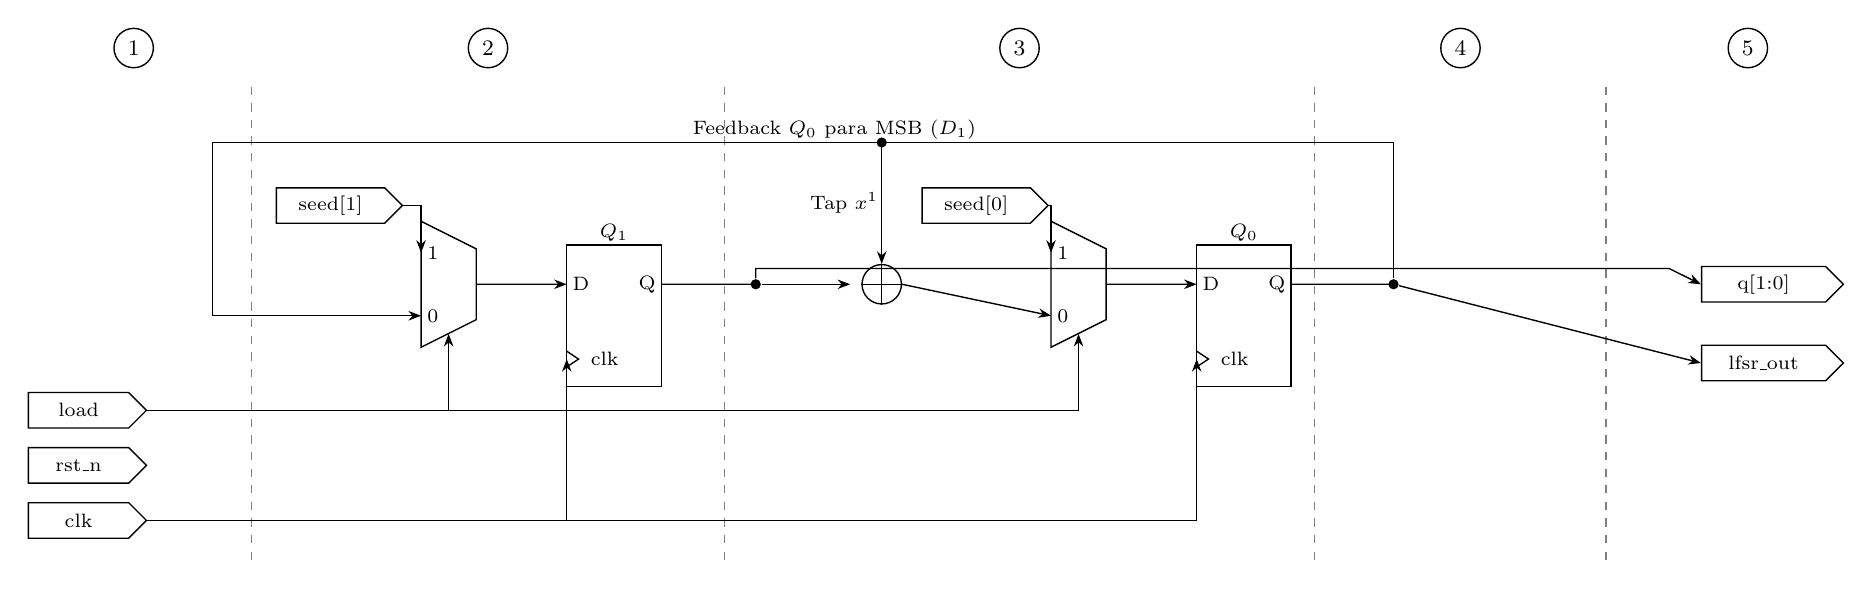
\begin{tikzpicture}[rtl]
  \Niveis{3.0, 9.0, 16.5, 20.2}{-2.5}{3.6}
  \NumNivel{1}{1.5}{4.0}
  \NumNivel{2}{6.0}{4.0}
  \NumNivel{3}{12.75}{4.0}
  \NumNivel{4}{18.35}{4.0}
  \NumNivel{5}{22.0}{4.0}

  \node[porta, minimum width=15mm] (p_clk)  at (0.8, -2.0) {clk};
  \node[porta, minimum width=15mm] (p_rst)  at (0.8, -1.3) {rst\_n};
  \node[porta, minimum width=15mm] (p_load) at (0.8, -0.6) {load};

  \node[porta, minimum width=16mm] (s1) at (4.0, 2.0) {seed[1]};
  \MUX{m1}{5.5, 1.0}
  \draw[->] (s1.east) -| (m1-in1);
  \FF{ff1}{7.6, 0.6}{$Q_1$}
  \draw[->] (m1-out) -- (ff1-d);

  \draw (ff1-q) -- (9.4, 1.0) node[no] (node_q1) {};
  \draw[->] (node_q1) -- (10.6, 1.0);

  \XOR{xor0}{11.0, 1.0}
  \node[porta, minimum width=16mm] (s0) at (12.2, 2.0) {seed[0]};
  \MUX{m0}{13.5, 1.0}
  \draw[->] (xor0.east) -- (m0-in0);
  \draw[->] (s0.east) -| (m0-in1);
  \FF{ff0}{15.6, 0.6}{$Q_0$}
  \draw[->] (m0-out) -- (ff0-d);

  \draw (ff0-q) -- (17.5, 1.0) node[no] (node_q0) {};
  \node[porta, minimum width=18mm] (p_q)   at (22.2, 1.0) {q[1:0]};
  \node[porta, minimum width=18mm] (p_out) at (22.2, 0.0) {lfsr\_out};

  \draw[->] (node_q1) |- (21.0, 1.2) -- (p_q.west);
  \draw[->] (node_q0) -- (p_out.west);

  \draw[->] (node_q0) |- (17.2, 2.8) -- (2.5, 2.8) |- (m1-in0);
  \node[barra, above] at (10.4, 2.8) {Feedback $Q_0$ para MSB ($D_1$)};

  \draw[->] (11.0, 2.8) node[no] {} -- node[barra, left] {Tap $x^1$} (xor0.north);

  \draw (p_clk.east) -- (15.0, -2.0);
  \draw[->] (7.0, -2.0) -- (ff1-clk);
  \draw[->] (15.0, -2.0) -- (ff0-clk);

  \draw (p_load.east) -- (13.5, -0.6);
  \draw[->] (5.5, -0.6) -- (m1-sel);
  \draw[->] (13.5, -0.6) -- (m0-sel);

\end{tikzpicture}
}
    \caption{RTL do LFSR Galois de 2 bits ($2^1$), polinômio primitivo $P(x) = x^2 + x + 1$ (Período Máximo = 3).}
  \end{subfigure}\\[2mm]
  \begin{subfigure}{\linewidth}\centering
    \resizebox{0.78\linewidth}{!}{% Autor: Matheus Sousa, Labotatório de Comunicação e Segurança da Informação, DES-CTG, UFPE.
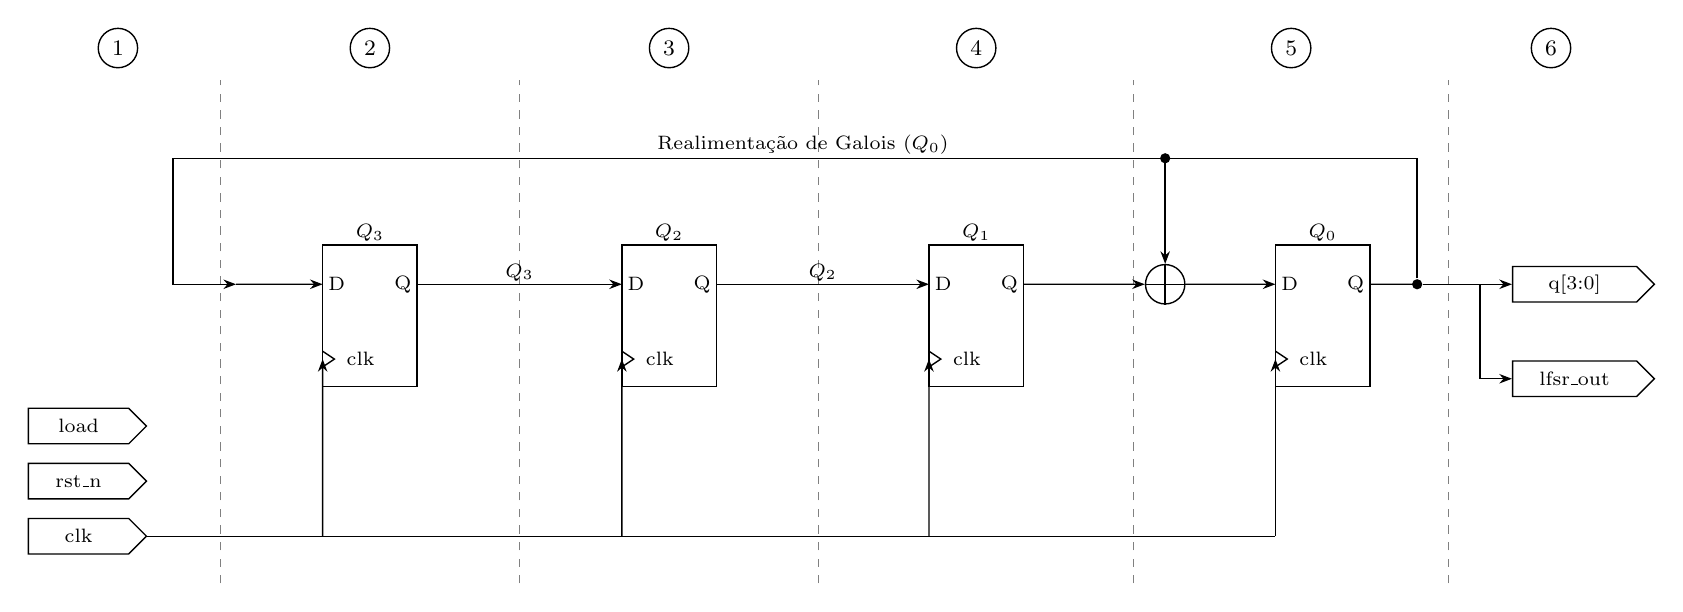
\begin{tikzpicture}[rtl]
  \Niveis{2.6, 6.4, 10.2, 14.2, 18.2}{-2.6}{3.8}
  \NumNivel{1}{1.3}{4.2}
  \NumNivel{2}{4.5}{4.2}
  \NumNivel{3}{8.3}{4.2}
  \NumNivel{4}{12.2}{4.2}
  \NumNivel{5}{16.2}{4.2}
  \NumNivel{6}{19.5}{4.2}

  \node[porta, minimum width=15mm] (clk)  at (0.8, -2.0) {clk};
  \node[porta, minimum width=15mm] (rst)  at (0.8, -1.3) {rst\_n};
  \node[porta, minimum width=15mm] (load) at (0.8, -0.6) {load};

  \FF{ff3}{4.5, 0.8}{$Q_3$}
  \draw[->] (2.8, 1.2) -- (ff3-d);

  \FF{ff2}{8.3, 0.8}{$Q_2$}
  \draw[->] (ff3-q) -- node[barra, above] {$Q_3$} (ff2-d);

  \FF{ff1}{12.2, 0.8}{$Q_1$}
  \draw[->] (ff2-q) -- node[barra, above] {$Q_2$} (ff1-d);

  \XOR{xor0}{14.6, 1.2}
  \draw[->] (ff1-q) -- (xor0.west);

  \FF{ff0}{16.6, 0.8}{$Q_0$}
  \draw[->] (xor0.east) -- (ff0-d);

  \draw (ff0-q) -- (17.8, 1.2) node[no] (node_fb) {};

  \draw[->] (node_fb) |- (17.5, 2.8) -- (2.0, 2.8) |- (2.8, 1.2);
  \node[barra, above] at (10.0, 2.8) {Realimentação de Galois ($Q_0$)};

  \draw[->] (14.6, 2.8) node[no] {} -- (xor0.north);

  \draw (clk.east) -- (16.0, -2.0);
  \draw[->] (3.9, -2.0) -- (ff3-clk);
  \draw[->] (7.7, -2.0) -- (ff2-clk);
  \draw[->] (11.6, -2.0) -- (ff1-clk);
  \draw[->] (16.0, -2.0) -- (ff0-clk);

  \node[porta, minimum width=18mm] (p_q)   at (19.8, 1.2) {q[3:0]};
  \node[porta, minimum width=18mm] (p_out) at (19.8, 0.0) {lfsr\_out};

  \draw[->] (node_fb) -| (18.6, 0.0) -- (p_out.west);
  \draw[->] (node_fb) -- (p_q.west);

\end{tikzpicture}
}
    \caption{RTL do LFSR Galois de 4 bits ($2^2$), polinômio primitivo $P(x) = x^4 + x + 1$ (Período Máximo = 15).}
  \end{subfigure}
  \caption{Esquemáticos RTL detalhados dos LFSRs de Galois para $N = 2$ e $N = 4$ bits.
    Em (a), o circuito possui apenas dois flip-flops e uma porta XOR no estágio LSB ($D_0 = Q_1 \oplus Q_0$),
    percorrendo a sequência cíclica de 3 estados não-nulos ($01 \to 11 \to 10$).
    Em (b), o registrador de 4 bits possui um único tap no bit 1 ($D_0 = Q_1 \oplus Q_0$),
    atingindo o período de 15 estados.}
  \label{fig:rtl_galois_2_4}
\end{figure}

\begin{figure}[p]
  \centering
  \begin{subfigure}{\linewidth}\centering
    \resizebox{0.82\linewidth}{!}{% Autor: Matheus Sousa, Labotatório de Comunicação e Segurança da Informação, DES-CTG, UFPE.
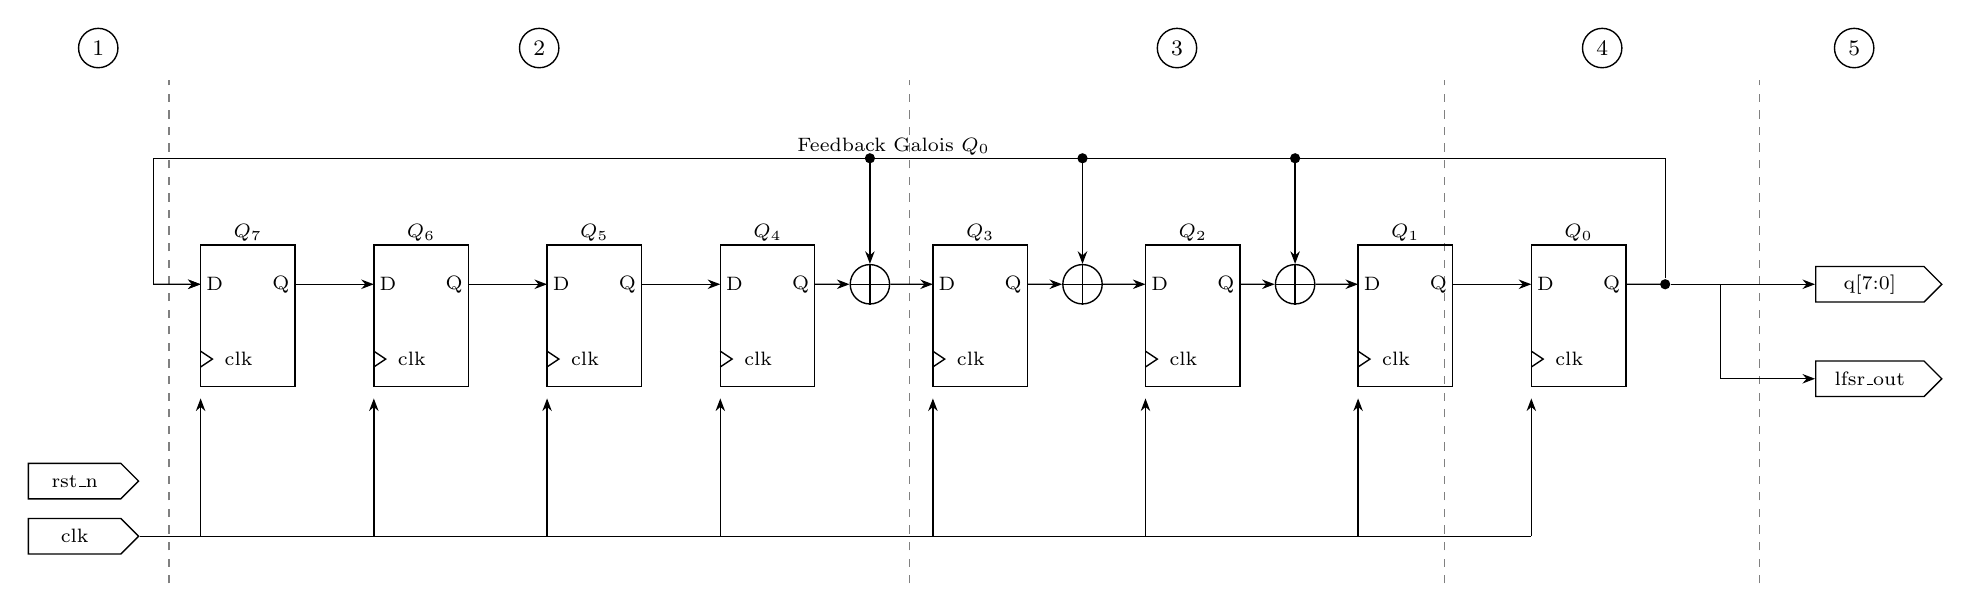
\begin{tikzpicture}[rtl]
  \Niveis{1.8, 11.2, 18.0, 22.0}{-2.6}{3.8}
  \NumNivel{1}{0.9}{4.2}
  \NumNivel{2}{6.5}{4.2}
  \NumNivel{3}{14.6}{4.2}
  \NumNivel{4}{20.0}{4.2}
  \NumNivel{5}{23.2}{4.2}

  \node[porta, minimum width=14mm] (clk)  at (0.6, -2.0) {clk};
  \node[porta, minimum width=14mm] (rst)  at (0.6, -1.3) {rst\_n};

  \FF{ff7}{2.8, 0.8}{$Q_7$}
  \FF{ff6}{5.0, 0.8}{$Q_6$}
  \FF{ff5}{7.2, 0.8}{$Q_5$}
  \FF{ff4}{9.4, 0.8}{$Q_4$}

  \draw[->] (1.6, 1.2) -- (ff7-d);
  \draw[->] (ff7-q) -- (ff6-d);
  \draw[->] (ff6-q) -- (ff5-d);
  \draw[->] (ff5-q) -- (ff4-d);

  \XOR{xor3}{10.7, 1.2}
  \draw[->] (ff4-q) -- (xor3.west);
  \FF{ff3}{12.1, 0.8}{$Q_3$}
  \draw[->] (xor3.east) -- (ff3-d);

  \XOR{xor2}{13.4, 1.2}
  \draw[->] (ff3-q) -- (xor2.west);
  \FF{ff2}{14.8, 0.8}{$Q_2$}
  \draw[->] (xor2.east) -- (ff2-d);

  \XOR{xor1}{16.1, 1.2}
  \draw[->] (ff2-q) -- (xor1.west);
  \FF{ff1}{17.5, 0.8}{$Q_1$}
  \draw[->] (xor1.east) -- (ff1-d);

  \FF{ff0}{19.7, 0.8}{$Q_0$}
  \draw[->] (ff1-q) -- (ff0-d);

  \draw (ff0-q) -- (20.8, 1.2) node[no] (node_fb) {};
  \draw[->] (node_fb) |- (20.5, 2.8) -- (1.6, 2.8) |- (ff7-d);
  \node[barra, above] at (11.0, 2.8) {Feedback Galois $Q_0$};

  \draw[->] (10.7, 2.8) node[no] {} -- (xor3.north);
  \draw[->] (13.4, 2.8) node[no] {} -- (xor2.north);
  \draw[->] (16.1, 2.8) node[no] {} -- (xor1.north);

  \draw (clk.east) -- (19.1, -2.0);
  \foreach \x in {2.2, 4.4, 6.6, 8.8, 11.5, 14.2, 16.9, 19.1} {
    \draw[->] (\x, -2.0) -- ++(0, 1.75);
  }

  \node[porta, minimum width=16mm] (p_q)   at (23.4, 1.2) {q[7:0]};
  \node[porta, minimum width=16mm] (p_out) at (23.4, 0.0) {lfsr\_out};

  \draw[->] (node_fb) -- (p_q.west);
  \draw[->] (node_fb) -| (21.5, 0.0) -- (p_out.west);

\end{tikzpicture}
}
    \caption{RTL do LFSR Galois de 8 bits ($2^3$), polinômio primitivo $P(x) = x^8 + x^4 + x^3 + x^2 + 1$ (Período Máximo = 255).}
  \end{subfigure}\\[2mm]
  \begin{subfigure}{\linewidth}\centering
    \resizebox{0.78\linewidth}{!}{% Autor: Matheus Sousa, Labotatório de Comunicação e Segurança da Informação, DES-CTG, UFPE.
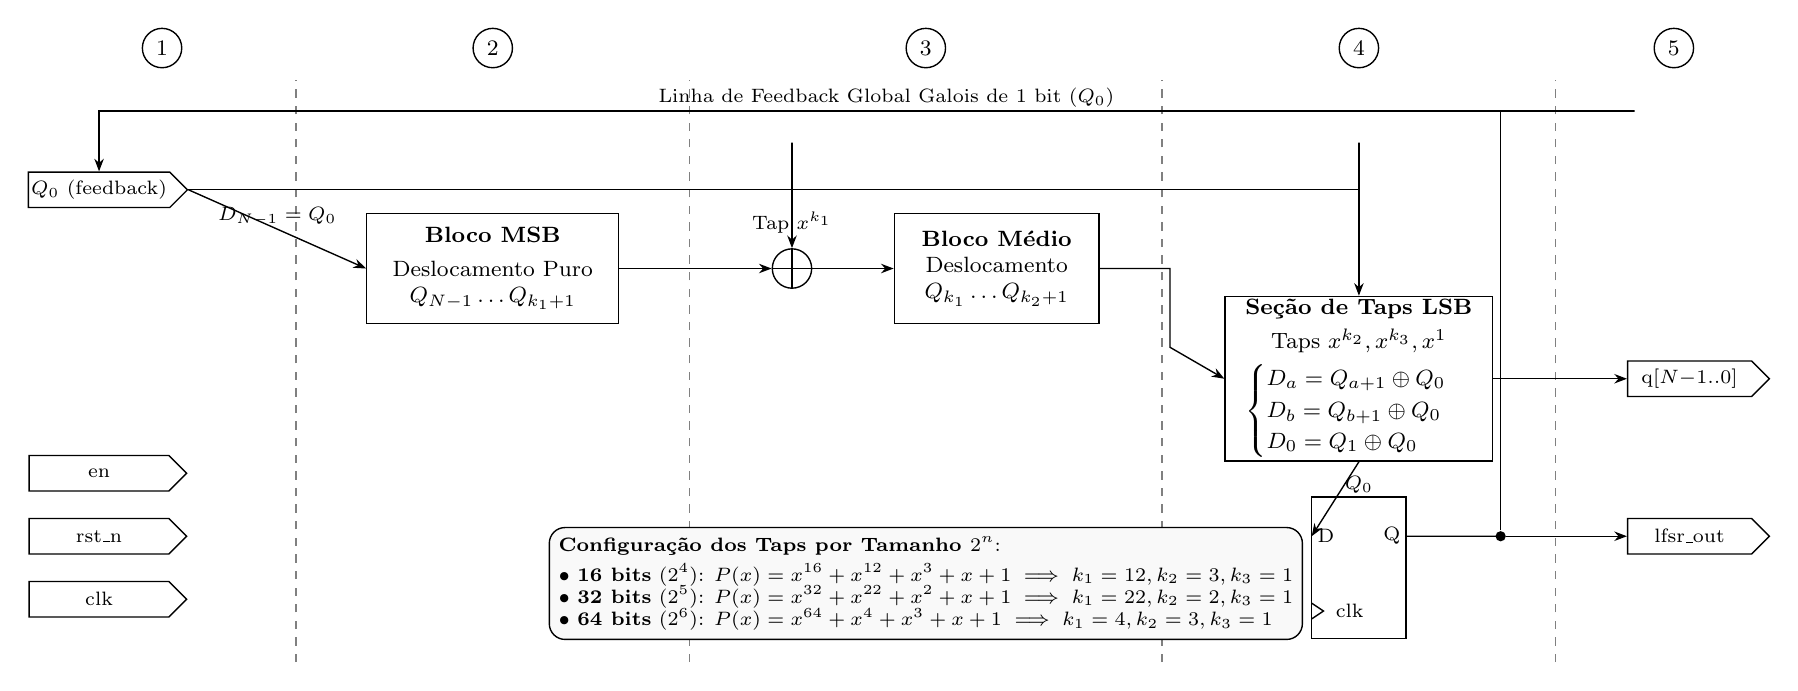
\begin{tikzpicture}[rtl]
  \Niveis{3.5, 8.5, 14.5, 19.5}{-3.2}{4.2}
  \NumNivel{1}{1.8}{4.6}
  \NumNivel{2}{6.0}{4.6}
  \NumNivel{3}{11.5}{4.6}
  \NumNivel{4}{17.0}{4.6}
  \NumNivel{5}{21.0}{4.6}

  \node[porta, minimum width=20mm] (clk) at (1.0, -2.4) {clk};
  \node[porta, minimum width=20mm] (rst) at (1.0, -1.6) {rst\_n};
  \node[porta, minimum width=20mm] (en)  at (1.0, -0.8) {en};
  \node[porta, minimum width=20mm] (fb_in) at (1.0, 2.8) {$Q_0$ (feedback)};

  \node[bloco, minimum width=32mm, minimum height=14mm] (b_msb) at (6.0, 1.8) {
    \textbf{Bloco MSB}\\[1mm]
    Deslocamento Puro\\
    $Q_{N-1} \dots Q_{k_1+1}$
  };
  \draw[->] (fb_in.east) -- node[barra, above] {$D_{N-1} = Q_0$} (b_msb.west);

  \XOR{xor_k1}{9.8, 1.8}
  \draw[->] (b_msb.east) -- (xor_k1.west);
  \draw[->] (fb_in.east) -| (9.8, 3.4) -- (xor_k1.north);
  \node[barra, above] at (9.8, 2.2) {Tap $x^{k_1}$};

  \node[bloco, minimum width=26mm, minimum height=14mm] (b_mid) at (12.4, 1.8) {
    \textbf{Bloco Médio}\\
    Deslocamento\\
    $Q_{k_1} \dots Q_{k_2+1}$
  };
  \draw[->] (xor_k1.east) -- (b_mid.west);

  \node[bloco, minimum width=34mm, minimum height=20mm] (b_taps) at (17.0, 0.4) {
    \textbf{Seção de Taps LSB}\\[1mm]
    Taps $x^{k_2}, x^{k_3}, x^1$\\[1mm]
    $\begin{cases}
      D_a = Q_{a+1} \oplus Q_0\\
      D_b = Q_{b+1} \oplus Q_0\\
      D_0 = Q_1 \oplus Q_0
    \end{cases}$
  };
  \draw[->] (b_mid.east) -| (14.6, 0.8) -- (b_taps.west);
  \draw[->] (fb_in.east) -| (17.0, 3.4) -- (b_taps.north);

  \FF{ff0}{17.0, -2.0}{$Q_0$}
  \draw[->] (b_taps.south) -- (ff0-d);

  \draw (ff0-q) -- (18.8, -1.6) node[no] (node_lfsr_out) {};
  \draw[->] (node_lfsr_out) |- (20.5, 3.8) -- (1.0, 3.8) -- (fb_in.north);
  \node[barra, above] at (11.0, 3.8) {Linha de Feedback Global Galois de $1$ bit ($Q_0$)};

  \node[porta, minimum width=18mm] (p_q)   at (21.2, 0.4) {q[$N{-}1..0$]};
  \node[porta, minimum width=18mm] (p_out) at (21.2, -1.6) {lfsr\_out};

  \draw[->] (b_taps.east) -- (p_q.west);
  \draw[->] (node_lfsr_out) -- (p_out.west);

  \node[draw, rounded corners=2mm, fill=gray!5, font=\scriptsize, align=left] at (11.5, -2.2) {
    \textbf{Configuração dos Taps por Tamanho $2^n$}:\\[1mm]
    $\bullet$ \textbf{16 bits} ($2^4$): $P(x) = x^{16} + x^{12} + x^3 + x + 1 \implies k_1=12, k_2=3, k_3=1$\\
    $\bullet$ \textbf{32 bits} ($2^5$): $P(x) = x^{32} + x^{22} + x^2 + x + 1 \implies k_1=22, k_2=2, k_3=1$\\
    $\bullet$ \textbf{64 bits} ($2^6$): $P(x) = x^{64} + x^4 + x^3 + x + 1 \implies k_1=4, k_2=3, k_3=1$
  };

\end{tikzpicture}
}
    \caption{Estrutura modular e mapeamento de taps dos LFSRs Galois de alta largura: 16 bits ($2^4$), 32 bits ($2^5$) e 64 bits ($2^6$).}
  \end{subfigure}
  \caption{Esquemáticos RTL dos geradores de ordem superior.
    Em (a), os três XORs intermediários correspondem aos expoentes $x^4, x^3, x^2$ do polinômio primitivo,
    garantindo que qualquer caminho combinacional contenha no máximo um atraso de porta XOR ($t_{cq} + t_{xor} + t_{setup}$).
    Em (b), visualização da organização modular em cascata com distribuição do sinal de feedback para os taps ótimos
    que atingem os períodos de $65.535$, $4.294.967.295$ e $18.446.744.073.709.551.615$ ciclos de clock.}
  \label{fig:rtl_galois_8_64}
\end{figure}

\end{document}
